
\subsection{Mesh Size}
\paragraph{}
The area of a subdomain will apparently influence the accuracy of the result.
Generally speaking, a larger subdomain tends to have a higher error.
The area of any polygon in fig.~\ref{adap_ei_polygon} can be calculated as 

\begin{equation}
    S = \frac{1}{2}
        \sum_{k=1}
        \left(
            x_k y_{k+1} - x_{k+1} y_k
        \right)
\end{equation}

\begin{figure}[!ht]
    \centering
    \scalebox{1}{
        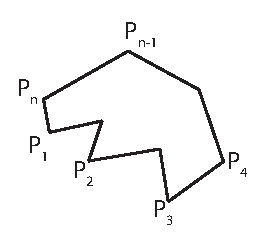
\includegraphics{adaptivity/images/adap_ei_polygon.eps}
    }
    \caption{A polygon with $n$ vertexes}
    \label{adap_ei_polygon}
\end{figure}

%   ----    %
\subsection{Mesh Quality}
\paragraph{}
Mesh quality is another important factor that influence the accuracy.
In SBFEM, mesh quality is highly related to the minimal angle formed by the intersecting lines connected by scaling center and adjacent polygon vertexes.
An extremely smaller angel may raise numerical stability issue and hence decrease the accuracy of the result.


%   ----    %

\subsection{Eigenvalue in SBFEM}
\paragraph{}
The displacement solution in SBFEM can be calculated as
\begin{equation}
    u(\xi)
\end{equation}


